\chapter{Difusión de partículas}\label{ch:b2:particle-diffusion}

Déjese caer un cristal de colorante en agua en reposo y obsérvese: se forma
a su alrededor una nube coloreada, crece, se ablanda por los bordes y se
extiende --- en un minuto por un milímetro, en una hora por un centímetro,
en una semana por todo el vaso. Nada empuja al colorante; lo lleva el
incesante zarandeo de las moléculas, que envía a cada partícula a un camino
aleatorio y, en promedio, de donde hay muchas a donde hay pocas.
Esto es la \emph{difusión}, el más lento y universal de los transportes:
alimenta de oxígeno a cada célula, dopa con boro cada transistor,
endurece el acero con carbono y deja que un perfume cruce una habitación --- aunque,
como veremos, no en el tiempo que uno pensaría. Este capítulo da a la
difusión su ley (Fick), su ecuación (a partir de un balance de partículas), sus
soluciones características y sus escalas de tiempo ($L \sim \sqrt{Dt}$), y su
origen microscópico en el camino aleatorio --- que también explica por qué la
\omterm{thm:b2:particle-diffusion:equation}{ecuación de difusión}, a diferencia de toda ecuación de la mecánica, conoce el
sentido del tiempo. El capítulo siguiente reutilizará todo ello para el calor.

\begin{omfigure}
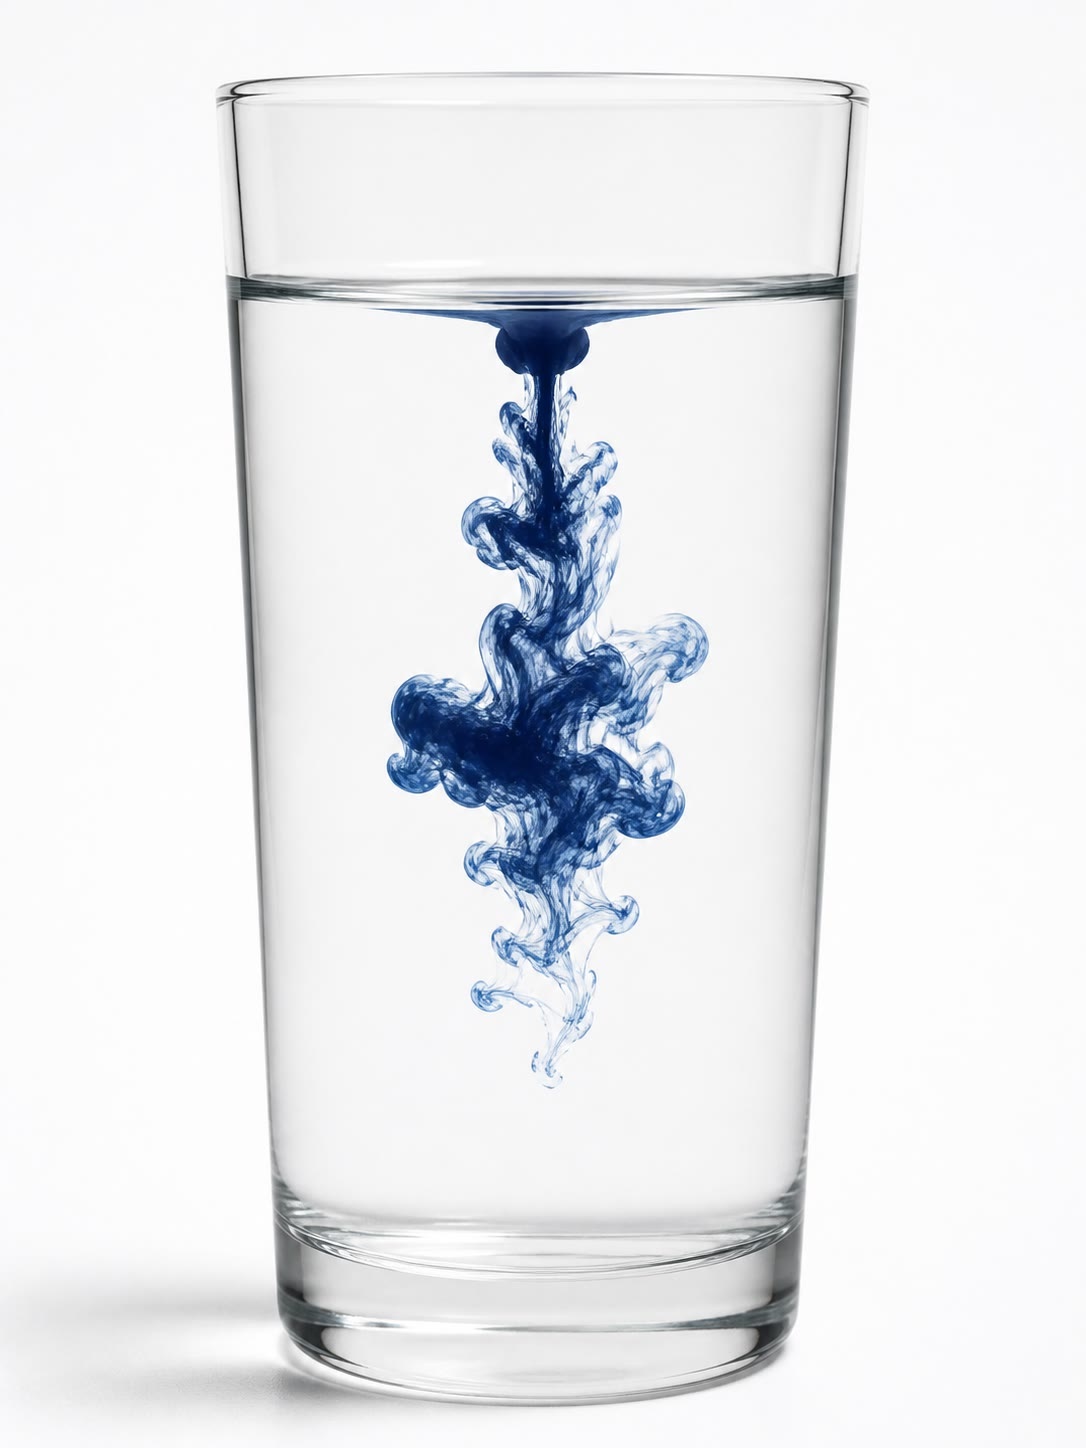
\includegraphics[width=0.58\linewidth]{images/book4/ai/b4-24-ink-drop-water.jpg}

{\small Tinta soltada en agua en reposo: la nube nítida se difumina y se extiende
a medida que sus moléculas difunden --- milímetros en un minuto, centímetros
en una hora.}
\end{omfigure}

\section{Densidad de partículas, flujo y ley de Fick}

\begin{definition}[Densidad y corriente de partículas]\label{def:b2:particle-diffusion:flux}
Para una especie de partículas (moléculas, iones, átomos en un sólido), la
\emph{densidad numérica}\index{densidad numérica} $n(M,t)$ es el número de
partículas por unidad de volumen en torno a $M$ (en \unit{m^{-3}}; la
concentración molar es $c = n/N_A$). La \emph{densidad de corriente de
partículas}\index{densidad de corriente de partículas} $\vect{j}_N$ es el vector
tal que el número de partículas que cruzan un elemento de superficie orientado
$\dd\vect S$ en $\dd t$ vale $\vect{j}_N\cdot\dd\vect S\,\dd t$ (en
\unit{m^{-2}.s^{-1}}): el \emph{flujo de partículas} a través de una superficie $S$ es
$\Phi_N = \iint_S \vect{j}_N\cdot\dd\vect S$, el número de partículas por
segundo a través de $S$. Para partículas arrastradas por un fluido que se mueve a $\vect v$,
$\vect{j}_N = n\vect v$ (convección); la difusión es el transporte que
queda en un fluido en reposo.
\end{definition}

\begin{theorem}[Ley de Fick]\label{thm:b2:particle-diffusion:fick}
En un medio en reposo, donde la densidad no es uniforme, aparece una
corriente de partículas proporcional y opuesta al \omterm{def:b2:maxwell-equations:operators}{gradiente} de la
densidad:
\[
\vect{j}_N = -D\,\vect{\operatorname{grad}}\,n ,
\]
donde el \emph{coeficiente de difusión}\index{coeficiente de difusión}
$D > 0$ (en \unit{m^2/s}) depende de la especie que difunde, del
medio y de la temperatura. Las partículas bajan \emph{a favor} del \omterm{def:b2:maxwell-equations:operators}{gradiente}
de densidad, de las regiones más densas a las más enrarecidas, a un ritmo que fija $D$.
\end{theorem}

\begin{proof}
Fenomenológica (una ley de la experiencia, como la de Ohm): lineal en el
\omterm{def:b2:maxwell-equations:operators}{gradiente} para \omterm{def:b2:maxwell-equations:operators}{gradientes} pequeños, isótropa en un medio isótropo y
con el signo que impone la experiencia. El modelo del camino aleatorio de
\cref{sec:b2:particle-diffusion:microscopic} la deduce, y con ella $D$,
a partir del movimiento molecular.
\end{proof}

\begin{example}[Órdenes de magnitud de $D$]\label{ex:b2:particle-diffusion:orders}
Gases: $D \sim \qty{1e-5}{m^2/s}$ (vapor de agua en aire,
\qty{2.5e-5}{m^2/s}; una molécula de perfume, \qty{5e-6}{m^2/s}). Líquidos:
$D \sim \qty{1e-9}{m^2/s}$ (oxígeno en agua, \qty{2e-9}{m^2/s}; azúcar,
\qty{5e-10}{m^2/s}; una proteína, \qty{1e-10}{m^2/s}). Sólidos: minúsculo y
con crecimiento abrupto con la temperatura, $D = D_0\,\eu^{-E_{\text{a}}/k_BT}$
(boro en silicio: \qty{1.5e-17}{m^2/s} a \qty{1100}{\celsius},
inmensurablemente pequeño a temperatura ambiente --- por eso un transistor,
una vez fabricado, conserva su perfil de dopado durante décadas). Cuatro órdenes de
magnitud del gas al líquido, y ocho o más del líquido al sólido.
\end{example}

\section{El balance de partículas y la ecuación de difusión}

\begin{theorem}[Balance local de partículas]\label{thm:b2:particle-diffusion:balance}
Si las partículas no se crean ni se destruyen,
\[
\frac{\partial n}{\partial t} + \operatorname{div}\vect{j}_N = 0 ;
\]
con una fuente que crea $\sigma$ partículas por unidad de volumen y tiempo
(una reacción química, una absorción), $\partial_t n +
\operatorname{div}\vect{j}_N = \sigma$. En una dimensión (con la densidad y la
corriente dependiendo solo de $x$): $\partial_t n + \partial_x j_N = 0$.
\end{theorem}

\begin{proof}
Tómese la rodaja entre $x$ y $x + \dd x$, de sección $S$: contiene
$n\,S\,\dd x$ partículas; en $\dd t$ entran $j_N(x)S\,\dd t$ por la
cara izquierda y salen $j_N(x + \dd x)S\,\dd t$ por la derecha, luego
$\partial_t n\,S\,\dd x\,\dd t = -(j_N(x+\dd x) - j_N(x))S\,\dd t =
-\partial_x j_N\,\dd x\,S\,\dd t$. En tres dimensiones, el mismo recuento en
una caja pequeña da la \omterm{def:b2:maxwell-equations:operators}{divergencia} (el flujo que sale de una superficie cerrada por
unidad de volumen, \cref{ch:b2:maxwell-equations}), o directamente: para todo
volumen fijo $V$, $\dd/\dd t \iiint_V n\,\dd\tau = -\iint_{\partial V}
\vect{j}_N\cdot\dd\vect S = -\iiint_V \operatorname{div}\vect{j}_N\,\dd\tau$
por el \omterm{thm:b2:maxwell-equations:theorems}{teorema de Ostrogradski}.
\end{proof}

\begin{omfigure}
\begin{tikzpicture}[scale=1.0, >=stealth]
  \draw[thick] (0,0) rectangle (5,2);
  \fill[omDef!12] (2.2,0) rectangle (2.9,2);
  \draw[omDef, thick] (2.2,0) -- (2.2,2);
  \draw[omDef, thick] (2.9,0) -- (2.9,2);
  \node[font=\scriptsize, below left] at (2.25,0) {$x$};
  \node[font=\scriptsize, below right] at (2.85,0) {$x + \dd x$};
  \draw[->, omExo, very thick] (1.0,1) -- (2.1,1) node[midway, above, font=\scriptsize] {$j_N(x)$};
  \draw[->, omExo, very thick] (3.0,1) -- (4.1,1) node[midway, above, font=\scriptsize] {$j_N(x + \dd x)$};
  \node[font=\scriptsize] at (2.55,1.6) {$n$};
  \node[font=\scriptsize, right] at (5.1,1) {sección $S$};
  \draw[->] (0,-0.7) -- (5.5,-0.7) node[right, font=\scriptsize] {$x$};
\end{tikzpicture}

{\small El balance unidimensional: la rodaja entre $x$ y $x + \dd
x$ gana lo que entra por la izquierda y pierde lo que sale por la derecha;
la diferencia es el cambio de $n$ en su interior.}
\end{omfigure}

\begin{theorem}[Ecuación de difusión]\label{thm:b2:particle-diffusion:equation}
Combinando la ley de Fick y el balance, para $D$ uniforme,
\[
\frac{\partial n}{\partial t} = D\,\Delta n + \sigma ,
\qquad\text{en una dimensión}\quad
\frac{\partial n}{\partial t} = D\,\frac{\partial^2 n}{\partial x^2} + \sigma .
\]
Esta \emph{ecuación de difusión}\index{ecuación de difusión} es lineal
(las soluciones se superponen), de primer orden en el tiempo y de segundo en el espacio
--- no es una \omterm{thm:b2:waves-on-strings:equation}{ecuación de ondas}: no tiene celeridad de propagación, sino una
relación característica entre longitud y tiempo,
\[
L \sim \sqrt{D t}, \qquad t \sim \frac{L^2}{D} :
\]
difundir el doble de distancia lleva cuatro veces más tiempo.
\end{theorem}

\begin{proof}
$\partial_t n = -\operatorname{div}(-D\,\vect{\operatorname{grad}}\,n) +
\sigma = D\operatorname{div}\vect{\operatorname{grad}}\,n + \sigma = D\Delta
n + \sigma$. Para las escalas, compárese $n/t$ con $Dn/L^2$.
\end{proof}

\begin{remark}[La difusión es irreversible]\label{rem:b2:particle-diffusion:irreversible}
Cámbiese $t$ por $-t$ en la \omterm{thm:b2:waves-on-strings:equation}{ecuación de ondas}, $\partial_t^2 u = c^2
\partial_x^2 u$, y no cambia: una película de una onda pasada al revés es
una onda posible. Hágase lo mismo en la \omterm{thm:b2:particle-diffusion:equation}{ecuación de difusión} y el signo del
miembro izquierdo se invierte: $n(x,-t)$ \emph{no} es solución. Una nube que
se extiende es natural; una nube que se reúne espontáneamente en un cristal
no lo es --- la difusión tiene una flecha del tiempo, la del segundo principio
(\cref{ch:b2:heat-conduction} calcula la entropía que crea). La
ecuación muestra además que la difusión suaviza: donde $n$ es localmente un
máximo ($\partial_x^2 n < 0$) disminuye, y donde es un mínimo,
aumenta.
\end{remark}

\begin{example}[¿Cuánto tarda?]\label{ex:b2:particle-diffusion:times}
$t \sim L^2/D$. Oxígeno a través de una célula, $L = \qty{10}{\micro m}$ en agua:
$10^{-10}/2 \times 10^{-9} = \qty{0.05}{s}$ --- la difusión alimenta una célula con
holgura; a través de \qty{1}{mm} de tejido: \qty{500}{s} --- demasiado lento, por lo que
nada vivo es más grueso que una fracción de milímetro sin
vasos sanguíneos. Azúcar por una taza de té sin remover, $L = \qty{5}{cm}$:
$2.5 \times 10^{-3}/5 \times 10^{-10} = 5 \times 10^6\,\unit{s}$, dos meses
--- remuévase. Un perfume por una habitación solo por difusión, \qty{5}{m} en
aire: $25/10^{-5} = \qty{3e6}{s}$, un mes; se huele en un minuto
porque el aire se mueve: la \emph{convección} transporta y la difusión solo
completa los últimos milímetros.
\end{example}

\section{Soluciones características}

\begin{proposition}[Régimen estacionario: la membrana]\label{prop:b2:particle-diffusion:membrane}
Entre dos depósitos mantenidos a $n_1$ y $n_2$, a través de una membrana de
espesor $e$ y área $S$, la densidad estacionaria es lineal,
\[
n(x) = n_1 + (n_2 - n_1)\frac{x}{e}, \qquad
j_N = D\,\frac{n_1 - n_2}{e}, \qquad
\Phi_N = \frac{n_1 - n_2}{R_{\text{d}}}, \quad R_{\text{d}} = \frac{e}{DS}:
\]
la membrana tiene una \emph{resistencia difusiva} $e/DS$, exactamente igual que un hilo
tiene $\ell/\gamma S$ --- las resistencias en serie se suman, y una membrana fina
de $D$ pequeño puede dominar aun así.
\end{proposition}

\begin{proof}
Estacionario, unidimensional y sin fuente: $\partial_x^2 n = 0$, luego $n$ es
afín; $j_N = -D\,\dd n/\dd x$ es uniforme.
\end{proof}

\begin{proposition}[Régimen estacionario: geometría esférica]\label{prop:b2:particle-diffusion:sphere}
En torno a una esfera de radio $a$ cuya superficie se mantiene a $n_0$, en un
medio donde $n \to 0$ lejos, la densidad estacionaria vale
\[
n(r) = n_0\,\frac{a}{r}, \qquad
\Phi_N = 4\pi D a\,n_0 :
\]
la corriente total liberada (o absorbida, con los signos invertidos) crece
con el \emph{radio}, no con la superficie, de la esfera --- la
geometría de un sumidero difusivo es la de una capacidad electrostática.
\end{proposition}

\begin{proof}
$\Delta n = \frac{1}{r^2}\frac{\dd}{\dd r}(r^2\,\dd n/\dd r) = 0$ da
$n = A + B/r$; las condiciones de contorno fijan $A = 0$, $B = n_0 a$; entonces
$\Phi_N = -4\pi r^2 D\,\dd n/\dd r = 4\pi D n_0 a$ para todo $r$ (sin
acumulación en régimen estacionario).
\end{proof}

\begin{omfigure}
\begin{tikzpicture}
  \begin{axis}[omaxis, width=5.6cm, height=4.2cm, xmin=-0.3, xmax=1.4, ymin=0, ymax=1.3,
    xlabel={$x/e$}, ylabel={$n/n_1$}, xtick={0,1}, ytick={1}, clip=false]
    \addplot[omDef, thick, domain=0:1] {1-0.7*x};
    \draw[dashed] (axis cs:1,0) -- (axis cs:1,0.3);
    \node[font=\scriptsize, anchor=west] at (axis cs:1.03,0.3) {$n_2$};
    \node[font=\scriptsize, omExo, anchor=west] at (axis cs:0.3,1.0) {$j_N = D(n_1 - n_2)/e$};
    \draw[->, omExo, thick] (axis cs:0.3,0.45) -- (axis cs:0.7,0.45);
  \end{axis}
  \begin{axis}[omaxis, width=5.6cm, height=4.2cm, xmin=0, xmax=5, ymin=0, ymax=1.3, xshift=5.9cm,
    xlabel={$r/a$}, ylabel={$n/n_0$}, xtick={1,2,3,4}, ytick={1}, clip=false]
    \addplot[omDef, thick, domain=1:5, samples=60] {1/x};
    \draw[dashed] (axis cs:1,0) -- (axis cs:1,1);
    \node[font=\scriptsize, omExo] at (axis cs:3,0.6) {$n = n_0 a/r$};
  \end{axis}
\end{tikzpicture}

{\small Perfiles estacionarios. A la izquierda, a través de una membrana la densidad es
lineal y la corriente uniforme. A la derecha, en torno a una esfera la densidad
cae como $1/r$; la corriente total $4\pi D a n_0$ es proporcional al
radio.}
\end{omfigure}

\begin{proposition}[La gaussiana que se extiende]\label{prop:b2:particle-diffusion:gaussian}
$N$ partículas por unidad de área soltadas en $t = 0$ en el plano $x = 0$ de
un medio infinito se extienden como
\[
n(x,t) = \frac{N}{\sqrt{4\pi D t}}\,\exp\Big(-\frac{x^2}{4Dt}\Big) :
\]
una gaussiana de desviación típica $\sigma(t) = \sqrt{2Dt}$, de área constante
$N$ (las partículas se conservan) y de pico decreciente $\propto
1/\sqrt t$. En tres dimensiones, $N$ partículas soltadas en un punto
se extienden como $n = N\,(4\pi Dt)^{-3/2}\exp(-r^2/4Dt)$, con $\langle r^2
\rangle = 6Dt$. Un pulso de partículas soltado en la \emph{superficie} de
un semiespacio (del que no pueden salir) da el doble de la expresión anterior
para $x > 0$.
\end{proposition}

\begin{proof}
Sustitúyase: con $u = x^2/4Dt$, $\partial_t n = n\,(-1/2t + u/t)$ y
$D\,\partial_x^2 n = D\,n\,(-1/2Dt + x^2/4D^2t^2) = n\,(-1/2t + u/t)$;
iguales. La normalización $\int n\,\dd x = N$ se sigue de $\int
\eu^{-x^2/4Dt}\dd x = \sqrt{4\pi Dt}$, y $\int x^2 n\,\dd x/N = 2Dt$.
La unicidad (dado el pulso inicial) se admite.
\end{proof}

\begin{omfigure}
\begin{tikzpicture}
  \begin{axis}[omaxis, width=9cm, height=4.8cm, xmin=-4.2, xmax=4.2, ymin=0, ymax=1.05,
    xlabel={$x/\sqrt{2Dt_1}$}, ylabel={$n$}, ytick=\empty, xtick={-4,-2,2,4}, clip=false,
    legend style={font=\scriptsize, at={(0.97,0.95)}, anchor=north east, draw=none, fill=none}]
    \addplot[omDef, thick, domain=-4.2:4.2, samples=100] {exp(-x*x/2)};
    \addlegendentry{$t_1$}
    \addplot[omThm, thick, domain=-4.2:4.2, samples=100] {0.5*exp(-x*x/8)};
    \addlegendentry{$4t_1$}
    \addplot[omExo, thick, domain=-4.2:4.2, samples=100] {0.25*exp(-x*x/32)};
    \addlegendentry{$16t_1$}
  \end{axis}
\end{tikzpicture}

{\small La solución gaussiana en tres instantes: la anchura crece como
$\sqrt t$, el pico cae como $1/\sqrt t$ y el área (el número de
partículas) no cambia.}
\end{omfigure}

\begin{proposition}[Concentración superficial constante]\label{prop:b2:particle-diffusion:erfc}
Un semiespacio $x > 0$ inicialmente vacío, cuya superficie se mantiene a la
densidad $n_0$ desde $t = 0$ (un gas en contacto con un sólido que
lo disuelve), se llena como
\[
n(x,t) = n_0\,\operatorname{erfc}\Big(\frac{x}{2\sqrt{Dt}}\Big),
\qquad
\operatorname{erfc}(u) = \frac{2}{\sqrt\pi}\int_u^{\infty}\eu^{-s^2}\dd s,
\]
la \emph{función error complementaria}, que cae de $1$ en $u =
0$ a $0.16$ en $u = 1$ y a $0.005$ en $u = 2$: la \omterm{def:b2:dispersion-wave-packets:complex}{profundidad de penetración} vale
de nuevo $\sim 2\sqrt{Dt}$, y el número total de partículas absorbidas por
unidad de área es $2n_0\sqrt{Dt/\pi}$.
\end{proposition}

\begin{proof}
Búsquese $n = f(u)$ con $u = x/2\sqrt{Dt}$: la ecuación se vuelve
$f'' + 2uf' = 0$, luego $f' \propto \eu^{-u^2}$ y $f$ es una función
error; las condiciones $f(0) = n_0$, $f(\infty) = 0$ seleccionan
$\operatorname{erfc}$. El número absorbido vale $\int_0^\infty n\,\dd x =
n_0\,2\sqrt{Dt}\int_0^\infty\operatorname{erfc}(u)\dd u = 2n_0\sqrt{Dt/\pi}$.
\end{proof}

\begin{example}[Endurecer el acero]\label{ex:b2:particle-diffusion:carburising}
Una pieza de acero mantenida a \qty{900}{\celsius} en un gas rico en carbono absorbe
carbono por su superficie; con $D = \qty{5e-12}{m^2/s}$ para el carbono en hierro
caliente, cuatro horas dan $2\sqrt{Dt} = \qty{0.5}{mm}$: una piel dura de medio
milímetro sobre un núcleo tenaz --- la \emph{cementación} de engranajes y
\omterm{def:b2:rigid-body-mechanics:pivot}{cojinetes}, cronometrada con el perfil de erfc.
\end{example}

\section{La imagen microscópica: el camino aleatorio}\label{sec:b2:particle-diffusion:microscopic}

\begin{proposition}[Camino aleatorio y coeficiente de difusión]\label{prop:b2:particle-diffusion:walk}
Una partícula que da un paso de longitud $\ell$ en una dirección al azar
cada $\tau$ (una molécula entre dos colisiones) tiene, tras $N =
t/\tau$ pasos, un desplazamiento cuadrático medio
\[
\langle x^2\rangle = N\ell^2 = \frac{\ell^2}{\tau}\,t
\quad\text{(una dimensión)}, \qquad
\langle r^2\rangle = 3\langle x^2\rangle \quad\text{(tres dimensiones)}.
\]
Comparando con la solución gaussiana, $\langle x^2\rangle = 2Dt$:
\[
D = \frac{\ell^2}{2\tau} \quad\text{(1D)}, \qquad
D = \frac{\ell^2}{6\tau} = \frac{\ell\,v^*}{6}\ \sim\ \frac{\ell\,v^*}{3}
\quad\text{(3D, con } v^* = \ell/\tau\text{; la teoría cinética da } \tfrac13) .
\]
La distancia del caminante crece como $\sqrt t$, no como $t$: para ir el doble de lejos
necesita cuatro veces más pasos.
\end{proposition}

\begin{proof}
$x = \sum_i \epsilon_i\ell$ con $\epsilon_i = \pm1$ independientes (1D):
$\langle x^2\rangle = \sum_{i,j}\langle\epsilon_i\epsilon_j\rangle\ell^2 =
N\ell^2$, pues los términos cruzados promedian cero. La distribución de $x$
para $N$ grande tiende a una gaussiana (el teorema central del límite, cuya
demostración corresponde al curso de probabilidad) --- por eso la
ley macroscópica es la \omterm{thm:b2:particle-diffusion:equation}{ecuación de difusión}; la propia ley de Fick se sigue
de contar los caminantes que cruzan un plano por ambos lados: $j_N \approx
-\tfrac12\ell v^*\,\partial_x n$ (un promedio más cuidadoso da $1/3$ en
tres dimensiones).
\end{proof}

\begin{omfigure}
\begin{tikzpicture}[scale=0.85]
  \draw[omDef, thin] plot coordinates {(0,0) (-0.1,-0.15) (-0.16,0.02) (-0.24,-0.14) (-0.1,-0.03) (-0.28,-0.05) (-0.46,-0.04) (-0.61,-0.14) (-0.73,-0.01) (-0.74,0.17) (-0.86,0.3) (-0.78,0.14) (-0.7,0.3) (-0.75,0.47) (-0.86,0.33) (-0.82,0.15) (-0.64,0.14) (-0.58,-0.03) (-0.76,0.01) (-0.93,-0.04) (-1.06,-0.16) (-1.06,0.02) (-1.11,-0.16) (-1.15,-0.33) (-0.97,-0.36) (-1.05,-0.2) (-1.22,-0.14) (-1.27,-0.31) (-1.28,-0.49) (-1.2,-0.33) (-1.02,-0.31) (-0.98,-0.49) (-0.81,-0.44) (-0.96,-0.55) (-0.95,-0.37) (-1.12,-0.43) (-1.3,-0.45) (-1.44,-0.34) (-1.37,-0.18) (-1.48,-0.32) (-1.52,-0.49) (-1.58,-0.32) (-1.4,-0.36) (-1.31,-0.51) (-1.45,-0.4) (-1.5,-0.57) (-1.37,-0.44) (-1.51,-0.56) (-1.68,-0.61) (-1.74,-0.78) (-1.59,-0.88) (-1.73,-0.77) (-1.64,-0.93) (-1.78,-1.05) (-1.6,-1.03) (-1.72,-0.91) (-1.59,-0.79) (-1.75,-0.86) (-1.88,-0.73) (-1.77,-0.58) (-1.71,-0.75) (-1.55,-0.67) (-1.39,-0.58) (-1.34,-0.41) (-1.19,-0.52) (-1.36,-0.57) (-1.54,-0.56) (-1.67,-0.43) (-1.53,-0.33) (-1.7,-0.28) (-1.76,-0.11) (-1.89,0.02) (-1.76,0.14) (-1.59,0.08) (-1.55,-0.09) (-1.71,-0.02) (-1.88,-0.09) (-1.7,-0.07) (-1.52,-0.11) (-1.43,0.04) (-1.53,0.19) (-1.53,0.01) (-1.57,-0.17) (-1.48,-0.33) (-1.4,-0.16) (-1.46,-0.33) (-1.29,-0.28) (-1.11,-0.29) (-0.93,-0.25) (-0.84,-0.1) (-0.66,-0.11) (-0.74,-0.27) (-0.56,-0.22) (-0.55,-0.04) (-0.67,-0.18) (-0.57,-0.03) (-0.42,-0.13) (-0.59,-0.06) (-0.47,-0.2) (-0.65,-0.2) (-0.56,-0.04) (-0.52,-0.22) (-0.34,-0.21) (-0.29,-0.39) (-0.34,-0.21) (-0.21,-0.08) (-0.18,0.09) (-0.35,0.15) (-0.34,0.33) (-0.35,0.15) (-0.39,-0.03) (-0.43,0.15) (-0.38,0.33) (-0.47,0.17) (-0.61,0.06) (-0.48,-0.06) (-0.44,0.11) (-0.32,0.25) (-0.49,0.18) (-0.31,0.17) (-0.47,0.24) (-0.6,0.37) (-0.44,0.44) (-0.48,0.61) (-0.5,0.43) (-0.47,0.61) (-0.58,0.75) (-0.74,0.84) (-0.87,0.96) (-0.83,0.79) (-0.67,0.69) (-0.8,0.56) (-0.98,0.59) (-1.14,0.51) (-1.27,0.38) (-1.27,0.2) (-1.12,0.1) (-1.27,0.2) (-1.38,0.35) (-1.21,0.4) (-1.37,0.47) (-1.54,0.52) (-1.46,0.68) (-1.56,0.53) (-1.4,0.45) (-1.36,0.27) (-1.19,0.22) (-1.03,0.13) (-0.86,0.06) (-0.96,-0.1) (-1.14,-0.09) (-1.26,-0.22) (-1.08,-0.26) (-0.92,-0.2) (-0.74,-0.16) (-0.81,0) (-0.95,-0.11) (-1.06,-0.26) (-0.92,-0.14) (-1.07,-0.24) (-1.23,-0.33) (-1.27,-0.51) (-1.12,-0.61) (-1.04,-0.77) (-1.07,-0.6) (-0.93,-0.49) (-0.94,-0.67) (-0.78,-0.75) (-0.93,-0.85) (-0.78,-0.94) (-0.6,-0.93) (-0.6,-1.11) (-0.73,-1.24) (-0.63,-1.39) (-0.72,-1.24) (-0.66,-1.41) (-0.66,-1.23) (-0.48,-1.21) (-0.34,-1.33) (-0.41,-1.49) (-0.35,-1.65) (-0.21,-1.54) (-0.04,-1.48) (0.14,-1.44) (0.11,-1.27) (-0.01,-1.4) (0.15,-1.31) (-0.03,-1.26) (0.13,-1.36) (0.12,-1.18) (0.29,-1.13) (0.42,-1) (0.44,-1.18) (0.6,-1.26) (0.68,-1.42) (0.51,-1.39) (0.47,-1.21) (0.49,-1.39) (0.59,-1.25) (0.69,-1.39) (0.87,-1.43) (0.75,-1.3) (0.73,-1.48) (0.59,-1.37) (0.61,-1.55) (0.54,-1.71) (0.37,-1.63) (0.52,-1.53) (0.67,-1.63) (0.78,-1.78) (0.75,-1.6) (0.79,-1.42) (0.83,-1.6) (0.68,-1.5) (0.56,-1.63) (0.68,-1.49) (0.84,-1.56) (0.97,-1.43) (1.11,-1.31) (1.08,-1.49) (1.02,-1.33) (1.13,-1.47) (0.95,-1.44) (0.9,-1.27) (1.01,-1.13) (0.98,-1.3) (0.86,-1.18) (0.78,-1.01) (0.69,-1.17) (0.87,-1.15) (0.98,-1.28) (1.13,-1.38) (1,-1.51) (1.13,-1.38) (1.17,-1.55) (1.23,-1.38) (1.19,-1.21) (1.29,-1.36) (1.43,-1.47) (1.42,-1.65) (1.28,-1.76) (1.13,-1.65) (1.03,-1.8) (1.2,-1.85) (1.16,-1.68) (0.99,-1.76) (1.1,-1.9) (1.11,-2.08) (0.93,-2.11) (1.01,-1.95) (0.99,-2.13) (0.81,-2.14) (0.98,-2.18) (0.85,-2.05) (1.03,-2.1) (1.04,-1.92) (1.18,-2.03) (1.36,-2.01) (1.54,-2.04) (1.37,-1.98) (1.53,-1.92) (1.37,-1.84) (1.51,-1.72) (1.45,-1.55) (1.6,-1.46) (1.75,-1.36) (1.86,-1.22) (1.81,-1.39) (1.98,-1.34) (1.94,-1.16) (1.8,-1.05) (1.85,-1.22) (2.03,-1.22) (1.91,-1.08) (1.83,-0.92) (1.72,-1.05) (1.79,-0.89) (1.74,-1.06) (1.57,-1.12) (1.39,-1.15) (1.23,-1.22) (1.41,-1.22) (1.36,-1.05) (1.18,-1.06) (1,-1.06) (1.09,-1.22) (1.08,-1.04) (1.25,-1.1) (1.33,-0.95) (1.3,-0.77) (1.31,-0.95) (1.28,-0.77) (1.14,-0.88) (1.04,-1.03) (0.95,-0.88) (1.08,-0.75) (1.22,-0.86) (1.26,-1.03) (1.08,-1.01) (1.12,-1.19) (0.95,-1.11) (1.12,-1.03) (1.17,-1.2) (1.27,-1.05) (1.26,-1.23) (1.44,-1.21) (1.42,-1.03) (1.3,-0.9) (1.38,-1.06) (1.56,-1.02) (1.6,-1.2) (1.76,-1.28) (1.6,-1.36) (1.46,-1.26) (1.55,-1.41) (1.61,-1.58) (1.79,-1.58) (1.73,-1.41) (1.61,-1.27) (1.65,-1.1) (1.8,-1.01) (1.66,-1.12) (1.52,-1.23) (1.36,-1.31) (1.48,-1.45) (1.3,-1.41) (1.34,-1.24) (1.33,-1.06) (1.16,-1.09) (1.1,-0.92) (1.12,-0.74) (1.04,-0.91) (1.04,-0.73) (0.93,-0.58) (0.97,-0.41) (0.81,-0.49) (0.65,-0.41) (0.65,-0.23) (0.7,-0.05) (0.55,-0.15) (0.73,-0.11) (0.82,-0.27) (0.92,-0.42) (0.87,-0.25) (1.05,-0.23) (1.08,-0.41) (1.19,-0.27) (1.22,-0.45) (1.39,-0.42) (1.57,-0.41) (1.39,-0.38) (1.38,-0.56) (1.36,-0.74) (1.27,-0.9) (1.44,-0.82) (1.26,-0.79) (1.4,-0.91) (1.33,-1.07) (1.2,-1.2) (1.03,-1.16) (0.86,-1.09) (0.75,-0.95) (0.57,-0.98) (0.75,-1.02) (0.81,-1.18) (0.69,-1.05) (0.86,-1.11) (0.74,-1.24) (0.6,-1.35) (0.43,-1.39) (0.27,-1.49) (0.43,-1.39) (0.58,-1.3) (0.4,-1.33) (0.46,-1.15) (0.51,-1.33) (0.44,-1.16) (0.54,-1.02) (0.49,-1.19) (0.58,-1.03) (0.44,-1.15) (0.46,-0.97) (0.64,-0.94) (0.82,-0.94) (0.91,-0.79) (0.92,-0.97) (0.75,-0.93) (0.59,-0.84) (0.62,-0.66) (0.6,-0.48) (0.53,-0.65) (0.45,-0.49) (0.62,-0.43) (0.62,-0.25) (0.66,-0.07) (0.5,-0.15) (0.62,-0.28) (0.44,-0.24) (0.27,-0.3) (0.28,-0.48) (0.39,-0.62)};
  \fill[omExo] (0,0) circle (2.5pt);
  \fill[omThm] (0.39,-0.62) circle (2.5pt);
  \draw[thin, gray] (0,0) -- (-2.4,1.2);
  \node[font=\scriptsize, omExo, anchor=east] at (-2.4,1.2) {inicio};
  \draw[thin, gray] (0.39,-0.62) -- (2.5,-1.3);
  \node[font=\scriptsize, omThm, anchor=west] at (2.5,-1.3) {tras $400$ pasos};
  \draw[<->, thin] (-2.3,-2.5) -- (2.3,-2.5) node[midway, below, font=\scriptsize] {$\sim \ell\sqrt N$};
\end{tikzpicture}

{\small Un camino aleatorio de $400$ pasos de longitud $\ell$: el caminante solo
se ha alejado unos $20\ell$ de su punto de partida --- la ley del $\sqrt N$ que
hace la difusión tan lenta en distancias largas y tan rápida en las cortas.}
\end{omfigure}

\begin{example}[De las moléculas a $D$]\label{ex:b2:particle-diffusion:kinetic}
Aire a temperatura ambiente: recorrido libre medio $\ell \approx \qty{70}{nm}$,
celeridad media $v^* \approx \qty{500}{m/s}$: $D \approx \ell v^*/3 =
\qty{1.2e-5}{m^2/s}$, como se mide. Para difundir \qty{1}{m}, una molécula
necesita $N = (L/\ell)^2 = 2 \times 10^{14}$ colisiones, es decir, $N\ell/v^*
\approx \qty{3e4}{s}$ --- ocho horas para un trayecto que haría en
\qty{2}{ms} si volara recto. En un líquido, una esfera de radio $a$
zarandeada por las moléculas obedece la relación de Stokes--Einstein $D =
k_BT/6\pi\eta a$ (Einstein, 1905): para el azúcar, $a \approx \qty{0.4}{nm}$
en agua, $D = \qty{5e-10}{m^2/s}$; para un grano de \qty{1}{\micro m},
$\qty{4e-13}{m^2/s}$, un desplazamiento de un micrómetro por segundo ---
el movimiento browniano que Perrin midió para contar el número de Avogadro. En
un sólido, un átomo salta a un sitio vecino solo cuando una fluctuación
térmica aporta la energía de activación: $D = D_0\,\eu^{-E_{\text{a}}/k_BT}$,
que se duplica cada pocas decenas de kelvin cerca de \qty{1000}{\celsius}.
\end{example}

\begin{method}[Estimaciones de difusión]\label{meth:b2:particle-diffusion:method}
(1) Identifíquese $D$ (gas $10^{-5}$, líquido $10^{-9}$, sólido de tipo Arrhenius).
(2) Tiempo o distancia: $t \sim L^2/D$, $L \sim \sqrt{Dt}$ (con el
$\sqrt{2Dt}$ exacto para la anchura gaussiana y $2\sqrt{Dt}$ para la profundidad de erfc).
(3) Estacionario: lineal en una lámina ($R_{\text{d}} = e/DS$), $1/r$ en torno a una
esfera ($\Phi = 4\pi D a\,\Delta n$), $\ln r$ en torno a un cilindro. (4)
Transitorio: gaussiana para un pulso, erfc para una superficie mantenida; superpóngase.
(5) Pregúntese si no domina la convección. (6) Comprobación microscópica:
$D \sim \ell v^*/3$.
\end{method}

\section{Ejercicios}

\begin{exercise}[$\star$]\label{exo:b2:particle-diffusion:1}
Tiempos de difusión $L^2/D$: un terrón de azúcar en el fondo de una taza de \qty{5}{cm}
($D = \qty{5e-10}{m^2/s}$); perfume por una habitación de \qty{5}{m} ($D =
\qty{5e-6}{m^2/s}$); oxígeno a través de \qty{1}{mm} de tejido y de una
célula de \qty{10}{\micro m} ($D = \qty{2e-9}{m^2/s}$). ¿Cuáles de ellos hace
realmente la difusión?
\end{exercise}

\begin{exercise}[$\star$]\label{exo:b2:particle-diffusion:2}
Una membrana de \qty{1}{\micro m} de espesor y \qty{1}{cm^2} de área, con $D =
\qty{1e-11}{m^2/s}$ en su interior, separa una disolución a \qty{1}{mol/m^3}
de agua pura. \omterm{def:b2:charges-currents-conduction:densities}{Densidad de corriente}, flujo molar y número de moléculas
por segundo; resistencia difusiva; y con dos membranas así en serie.
\end{exercise}

\begin{exercise}[$\star$]\label{exo:b2:particle-diffusion:3}
Se suelta en agua una capa fina de colorante ($N = \qty{1e20}{m^{-2}}$),
$D = \qty{1e-9}{m^2/s}$. Anchura $\sqrt{2Dt}$ y densidad de pico tras
\qty{1}{s}, \qty{1}{h} y un día. ¿Cuándo ha caído el pico al
$1\%$ de su valor a \qty{1}{s}?
\end{exercise}

\begin{exercise}[$\star$]\label{exo:b2:particle-diffusion:4}
Moléculas del aire: $\ell = \qty{70}{nm}$, $v^* = \qty{500}{m/s}$. Estímese
$D$; número de colisiones y tiempo para difundir \qty{1}{m}; compárese con
el vuelo recto. Lo mismo para una molécula en agua ($\ell \approx
\qty{0.1}{nm}$, $v^* \approx \qty{500}{m/s}$): ¿es correcta la estimación, y
por qué no exactamente?
\end{exercise}

\begin{exercise}[$\star\star$]\label{exo:b2:particle-diffusion:5}
\emph{Oxígeno en un tejido.} Una lámina de tejido de espesor $2a$ consume
oxígeno al ritmo uniforme $q$ (por unidad de volumen); sus dos caras se
mantienen a $n_0$. (a) Escríbase la ecuación estacionaria con el sumidero y resuélvase.
(b) Condición para que el oxígeno llegue al centro. (c) $D = \qty{2e-9}{m^2/s}$,
$n_0 = \qty{0.2}{mol/m^3}$, $q = \qty{0.01}{mol/m^3/s}$: $a$ máximo. (d)
Conclúyase sobre la separación entre capilares.
\end{exercise}

\begin{exercise}[$\star\star$]\label{exo:b2:particle-diffusion:6}
\emph{Un grano que se disuelve.} Una esfera de azúcar de radio $a = \qty{1}{mm}$
en agua en reposo mantiene su superficie a la densidad de saturación $n_{\text{s}}
= \qty{5800}{mol/m^3}$; lejos, el agua es pura; $D =
\qty{5e-10}{m^2/s}$. (a) Perfil estacionario y corriente total. (b)
Número de moles del grano (densidad \qty{1590}{kg/m^3}, masa molar
\qty{342}{g/mol}) y tiempo de disolución (tómese la corriente constante).
(c) ¿Por qué es mayor el tiempo real, y por qué ayuda tanto remover?
(d) Muéstrese que para un cilindro muy largo el perfil estacionario es
logarítmico y el problema no tiene solución en un medio infinito.
\end{exercise}

\begin{exercise}[$\star\star$]\label{exo:b2:particle-diffusion:7}
\emph{Conservación e irreversibilidad.} (a) A partir de la ecuación, muéstrese
que $\int n\,\dd x$ es constante y que $\dd\langle x^2\rangle/\dd t =
2D$ (intégrese por partes, con $n \to 0$ en el infinito). (b) Muéstrese que
$n(x,-t)$ no satisface la ecuación. (c) ¿En qué se convierte la
solución gaussiana para $t < 0$? (d) Muéstrese que $\int n^2\,\dd x$ solo puede
decrecer: la difusión aplana.
\end{exercise}

\begin{exercise}[$\star\star$]\label{exo:b2:particle-diffusion:8}
\emph{Cementación.} Carbono en hierro caliente, $D = \qty{5e-12}{m^2/s}$ a
\qty{900}{\celsius}; superficie mantenida a $n_0$. (a) Compruébese que $n_0
\operatorname{erfc}(x/2\sqrt{Dt})$ resuelve la ecuación. (b) Profundidad a la
que $n = 0.1\,n_0$ tras \qty{4}{h} ($\operatorname{erfc}(1.16) = 0.1$).
(c) Tiempo para el doble de profundidad. (d) A \qty{950}{\celsius}, $D$ es $2.5$
veces mayor: tiempo ahorrado.
\end{exercise}

\begin{exercise}[$\star\star$]\label{exo:b2:particle-diffusion:9}
\emph{Stokes--Einstein.} $D = k_BT/6\pi\eta a$, agua con $\eta =
\qty{1e-3}{Pa.s}$, \qty{300}{K}. (a) $D$ para $a = \qty{1}{\micro m}$ y
desplazamiento cuadrático medio en \qty{1}{s} y en \qty{1}{min}. (b) $D$
para una proteína, $a = \qty{3}{nm}$. (c) El azúcar tiene $D = \qty{5e-10}{m^2/s}$:
radio efectivo. (d) ¿Cómo da el número de Avogadro medir $\langle x^2\rangle$ de un grano
al microscopio?
\end{exercise}

\begin{exercise}[$\star\star\star$]\label{exo:b2:particle-diffusion:10}
\emph{Tiempo de retardo de una membrana.} Una membrana de espesor $e$, inicialmente
vacía, se expone por una cara a $n_1$ en $t = 0$, con la otra cara mantenida
a $0$. (a) ¿Cuál es el flujo estacionario final? (b) Arguméntese que el flujo
en la cara lejana sube en un tiempo $\sim e^2/D$ (el retardo exacto vale
$e^2/6D$). (c) Un parche de medicamento con $e = \qty{20}{\micro m}$, $D =
\qty{1e-13}{m^2/s}$ a través de la capa externa de la piel: tiempo de retardo. (d) ¿Por qué
es útil el retardo para medir $D$, y el flujo estacionario para medir
$D \times$ solubilidad?
\end{exercise}

\begin{exercise}[$\star\star\star$]\label{exo:b2:particle-diffusion:11}
\emph{El absorbente perfecto.} Una esfera de radio $a$ absorbe toda
partícula que la toca, en un medio a $n_\infty$ lejos. (a)
Perfil estacionario y corriente total capturada. (b) Una bacteria, $a =
\qty{1}{\micro m}$, en una disolución de azúcar a $n_\infty = \qty{6e20}{m^{-3}}$,
$D = \qty{5e-10}{m^2/s}$: moléculas capturadas por segundo. (c) Su
superficie está cubierta por $N_{\text{r}}$ receptores absorbentes pequeños de
radio $s$, siendo el resto reflectante: cada receptor por separado captura $\approx
4Ds n_\infty$ (un disco); muéstrese que la célula entera captura casi el
máximo en cuanto $N_{\text{r}} s \gg a$, es decir, con una fracción minúscula de su
superficie cubierta. (d) Coméntese: por qué pueden permitirse las células miles de
receptores distintos.
\end{exercise}

\begin{exercise}[$\star\star\star$]\label{exo:b2:particle-diffusion:12}
\emph{Resolverla en una malla.} Divídase el espacio en celdas de tamaño $\Delta x$
y el tiempo en pasos $\Delta t$; escríbase $n_i^{k+1} = n_i^k + \alpha\,(n_{i+1}^k
- 2n_i^k + n_{i-1}^k)$ con $\alpha = D\Delta t/\Delta x^2$. (a) Justifíquese
a partir de la ecuación. (b) Interprétese como un camino aleatorio cuando $\alpha =
1/2$. (c) Muéstrese que para $\alpha > 1/2$ una densidad que alterna $+,-,+,-$
de celda en celda crece: inestabilidad. (d) Para el perfil de boro del
problema siguiente ($D = \qty{1.5e-17}{m^2/s}$, $\Delta x = \qty{10}{nm}$),
el mayor $\Delta t$ estable y el número de pasos para una hora.
\end{exercise}

\section{Problema: una oblea dopada y una habitación perfumada}

\begin{problem}[{Problema de fin de semana --- difusión en un sólido y en un gas}]\label{pb:b2:particle-diffusion:1}
\textbf{Parte I --- Redistribución del boro en silicio.}
El boro difunde en el silicio con $D = D_0\,\eu^{-E_{\text{a}}/k_BT}$, $D_0 =
\qty{7.6e-5}{m^2/s}$, $E_{\text{a}} = \qty{3.46}{eV}$; $k_B =
\qty{8.62e-5}{eV/K}$. Una dosis $Q = \qty{1e18}{m^{-2}}$ de boro se ha
depositado en una capa muy fina en la superficie de una oblea cuyo
dopado de fondo vale $n_B = \qty{1e21}{m^{-3}}$; después se calienta
(``redistribución'') a \qty{1100}{\celsius} durante una hora. La superficie
refleja el boro (no se escapa).
\begin{enumerate}
  \item Calcúlese $D$ a \qty{1100}{\celsius} y a \qty{1000}{\celsius}.
        ¿En qué factor cambia en esos \qty{100}{K}?
  \item ¿Por qué es el perfil tras la redistribución $n(x,t) = (Q/\sqrt{\pi
        Dt})\exp(-x^2/4Dt)$ y no la gaussiana de
        \cref{prop:b2:particle-diffusion:gaussian}? Compruébese que su
        integral sobre $x > 0$ vale $Q$.
  \item Concentración en la superficie tras una hora.
  \item La \emph{profundidad de unión} $x_j$ es donde $n = n_B$: calcúlese.
  \item ¿Cómo cambia $x_j$ si la redistribución dura cuatro horas?
        (Cuidado: la concentración superficial también cambia.)
  \item Cambio relativo de $D$ para un error de \qty{10}{K} en temperatura;
        control de temperatura necesario para tener $x_j$ al \qty{1}{\%}.
  \item A temperatura ambiente, $D$: estímese el tiempo que tarda el perfil en
        moverse una distancia atómica y conclúyase.
\end{enumerate}

\textbf{Parte II --- La predeposición.}
La dosis misma se introdujo a \qty{950}{\celsius} a partir de un gas que mantiene
la superficie en el límite de solubilidad $n_0 = \qty{2e26}{m^{-3}}$ durante
\qty{30}{min}.
\begin{enumerate}[resume]
  \item $D$ a \qty{950}{\celsius} y $\sqrt{Dt}$ para \qty{30}{min}.
  \item Perfil al final de la predeposición; profundidad a la que $n =
        n_B$ ($\operatorname{erfc}(3.2) \approx 6 \times 10^{-6}$).
  \item Dosis introducida; compárese con la $Q$ de la Parte I.
  \item ¿Por qué se predeposita a temperatura más baja y se redistribuye a
        temperatura más alta?
  \item Justifíquese que durante la redistribución la capa predepositada puede
        tratarse como infinitamente fina.
\end{enumerate}

\textbf{Parte III --- Un perfume en una habitación.}
Una gota de perfume (\qty{1}{mg}, masa molar \qty{150}{g/mol}) se evapora
de golpe en el rincón de una habitación en calma a \qty{300}{K} y \qty{1}{bar}.
Tómese el diámetro de colisión de la molécula de perfume con el aire como $d =
\qty{0.5}{nm}$ y la \omterm{def:b2:particle-diffusion:flux}{densidad numérica} del aire como $n_{\text{a}} = P/k_BT$.
\begin{enumerate}[resume]
  \item Número de moléculas liberadas; \omterm{def:b2:particle-diffusion:flux}{densidad numérica} del aire.
  \item Recorrido libre medio $\ell = 1/(\sqrt2\,\pi d^2 n_{\text{a}})$ de la
        molécula de perfume y su celeridad media $v^* = \sqrt{8RT/\pi M}$.
  \item Estímese $D = \ell v^*/3$.
  \item Tiempo para difundir \qty{5}{m}; ¿y si el aire deriva a
        \qty{0.1}{m/s}?
  \item Escríbase la gaussiana tridimensional de la nube (en un rincón:
        las paredes reflejan, multiplíquese por $8$). En un punto a \qty{1}{m},
        ¿en qué instante es máxima la concentración?
  \item \omterm{def:b2:particle-diffusion:flux}{Densidad numérica} máxima allí; compárese con un umbral de percepción
        de \qty{1e13}{m^{-3}}.
  \item El borde de la nube: ¿a qué distancia vale la densidad $10^{-6}$ de
        su valor central tras un día?
  \item Número de colisiones que sufre una molécula de perfume en un día.
\end{enumerate}

\textbf{Parte IV --- El caminante y la flecha del tiempo.}
\begin{enumerate}[resume]
  \item Un caminante da $N$ pasos $\pm\ell$ sobre una recta: desplazamiento medio y
        cuadrático medio; muéstrese que $\langle x^2\rangle = 2Dt$
        identifica $D = \ell^2/2\tau$.
  \item Probabilidad de que el caminante vuelva exactamente a su punto de partida tras
        $N = 2$, $4$ y $6$ pasos; coméntese la tendencia.
  \item Fílmese una nube que difunde y pásese la película al revés: ¿qué se
        ve y qué ecuación se viola?
  \item Explíquese en un párrafo cómo el movimiento reversible de las moléculas
        produce la \omterm{thm:b2:particle-diffusion:equation}{ecuación de difusión} irreversible.
  \item Resúmase: la escala de longitud, la escala de tiempo y la única
        magnitud que distingue un gas, un líquido y un sólido caliente.
\end{enumerate}
\end{problem}
